\RequirePackage[l2tabu, orthodox]{nag}
\documentclass{article}

\usepackage[letterpaper, margin=1.3cm]{geometry}
\usepackage{siunitx}
\usepackage{multicol}
\usepackage{mathtools}
\usepackage{amssymb}
\usepackage{mathrsfs}
\usepackage{graphicx}
\usepackage{float}
\usepackage[outputdir=obj]{minted}
\usepackage{pdflscape}
\usepackage{caption}
\usepackage{subcaption}
\usepackage{epstopdf}
\usepackage{filecontents}

\epstopdfsetup{outdir=./obj/}
\usemintedstyle{emacs}
\setminted{linenos,breaklines}
\begin{document}

\begin{titlepage}
    \begin{center}
        \vspace*{1cm}

        \huge{\textbf{Lab 5}}

        \vspace{0.5cm}

        \LARGE{FIR Filters}
        \vspace{5cm}

        \Large{\textbf{Michael Kwok (1548454)}}

        \vfill
        ECE 340 Discrete Time Signals and Systems\\
        Department of Electrical and Computer Engineering\\
        University of Alberta\\
        24 November 2020
    \end{center}
\end{titlepage}
\section{Audio Filtering}

\subsection{Low Pass Filter}

\begin{figure}[H]
    \centering
    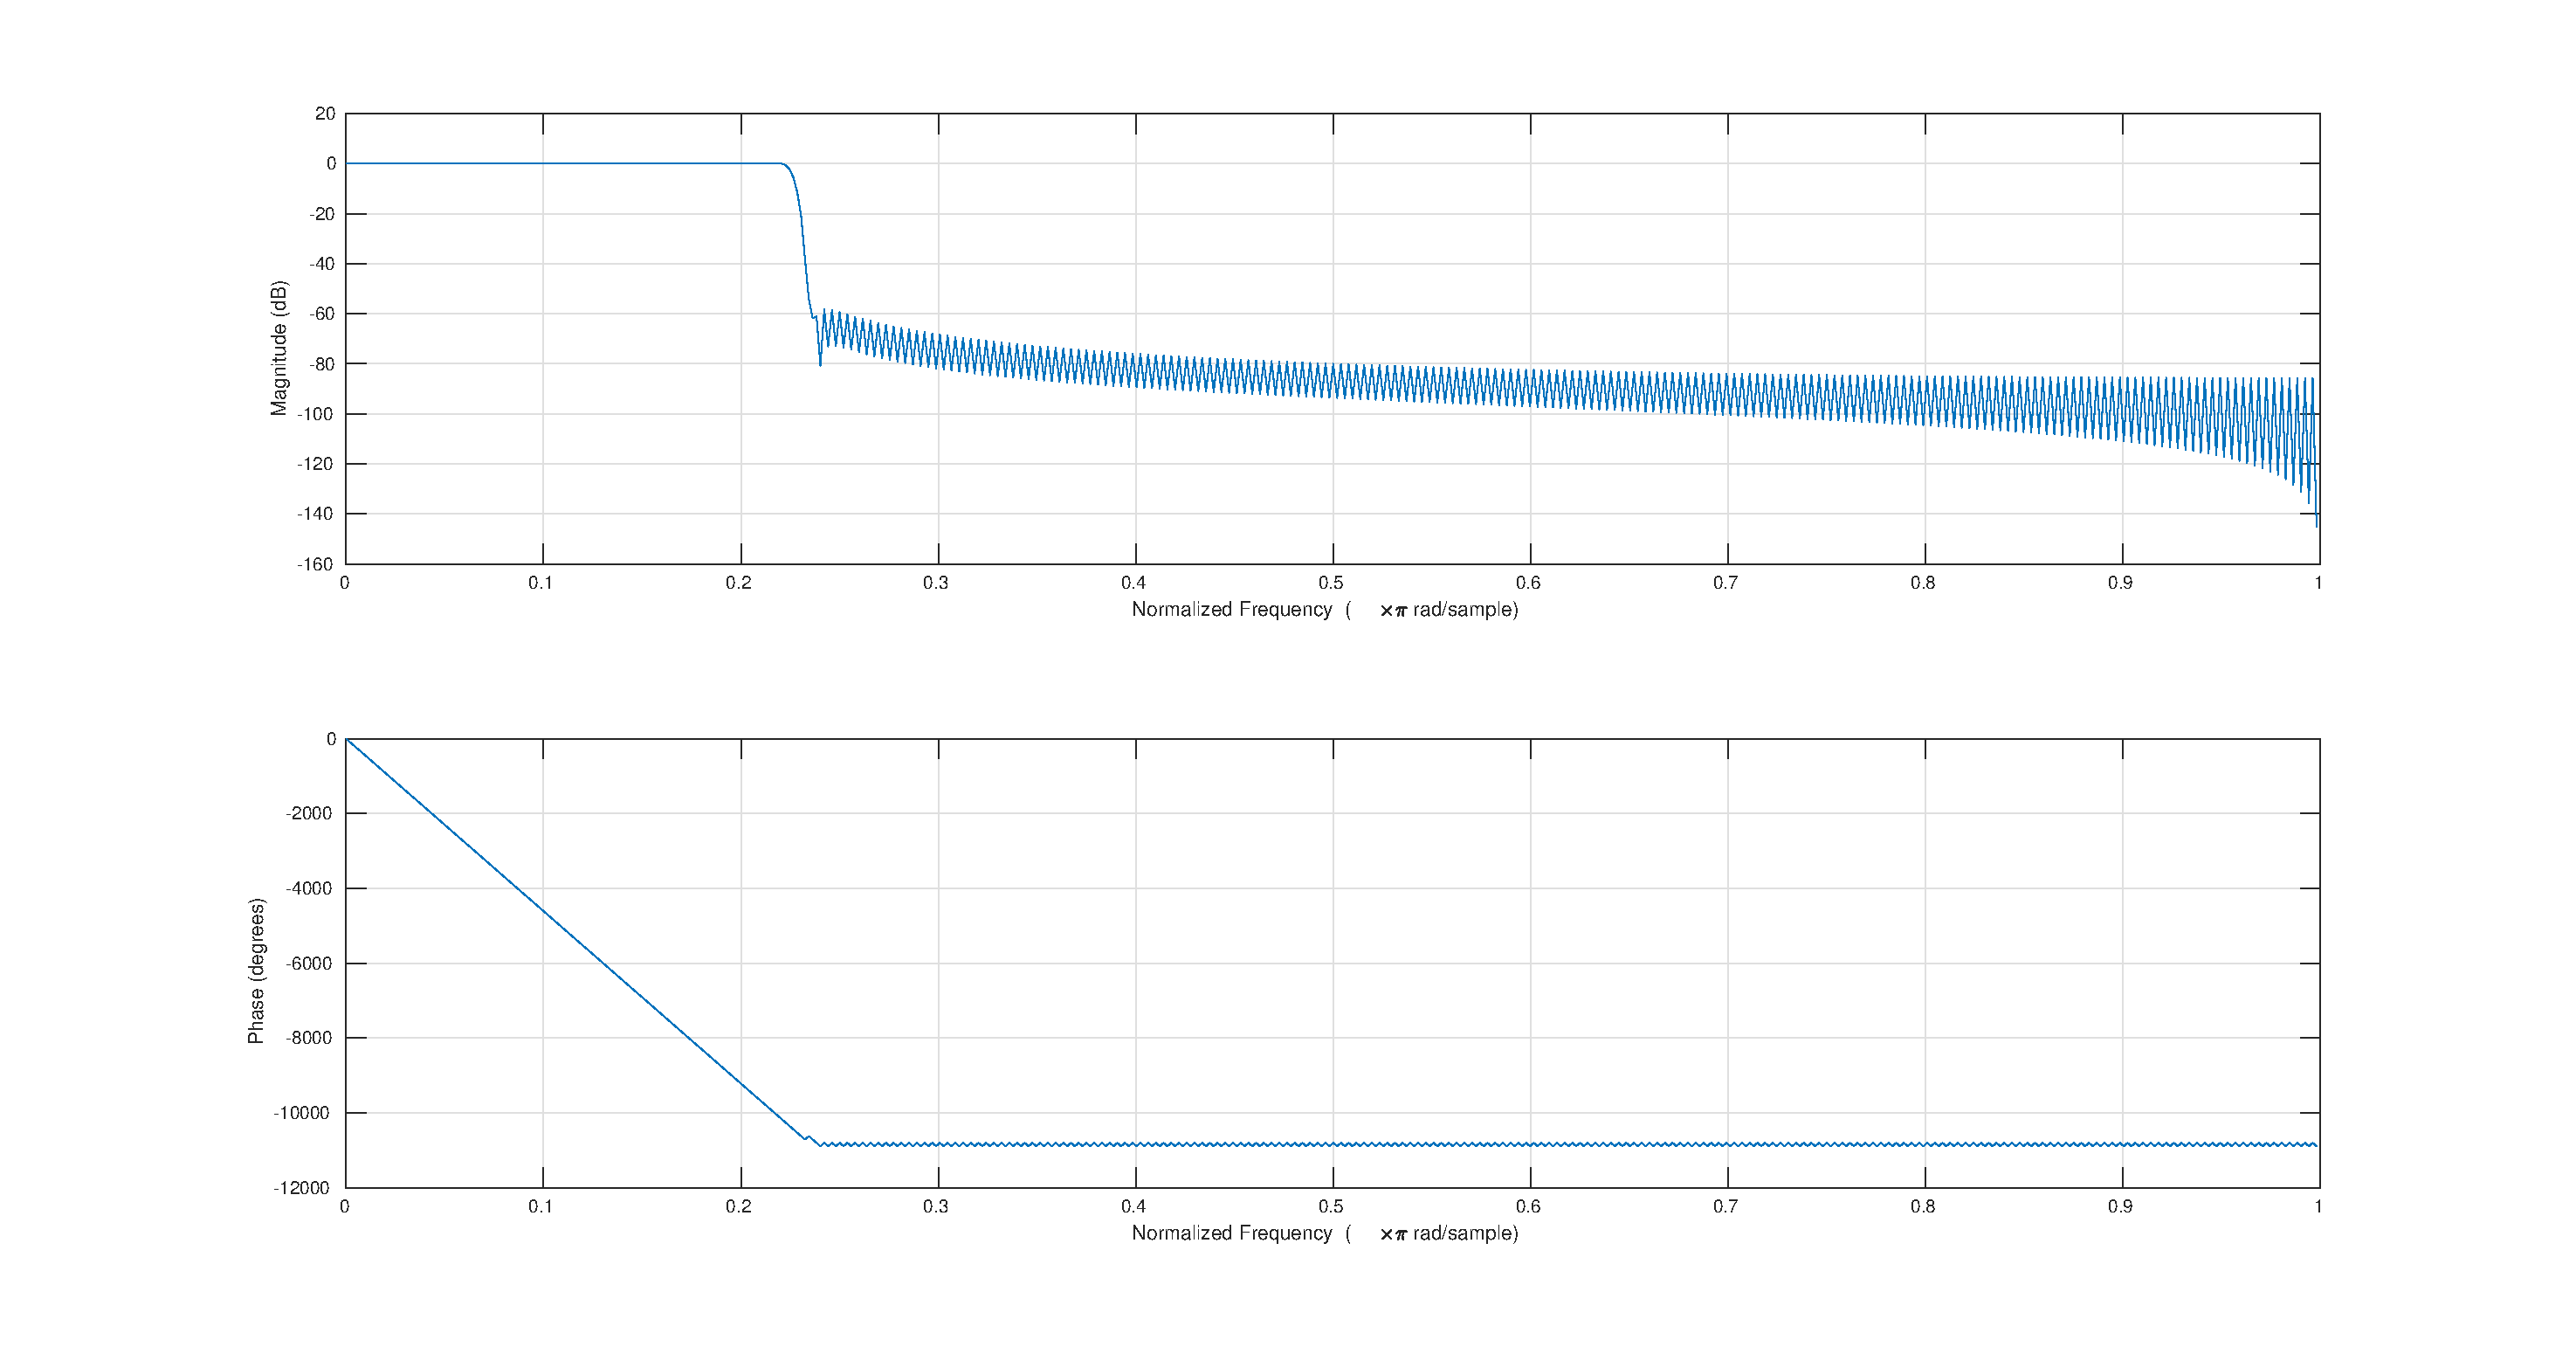
\includegraphics[width=\textwidth]{hamming_lps}
    \caption{Frequency response of Filter}
    \label{fig:filt1}
\end{figure}

\begin{figure}[H]
    \centering
    \begin{subfigure}[b]{0.45\textwidth}
        \centering
        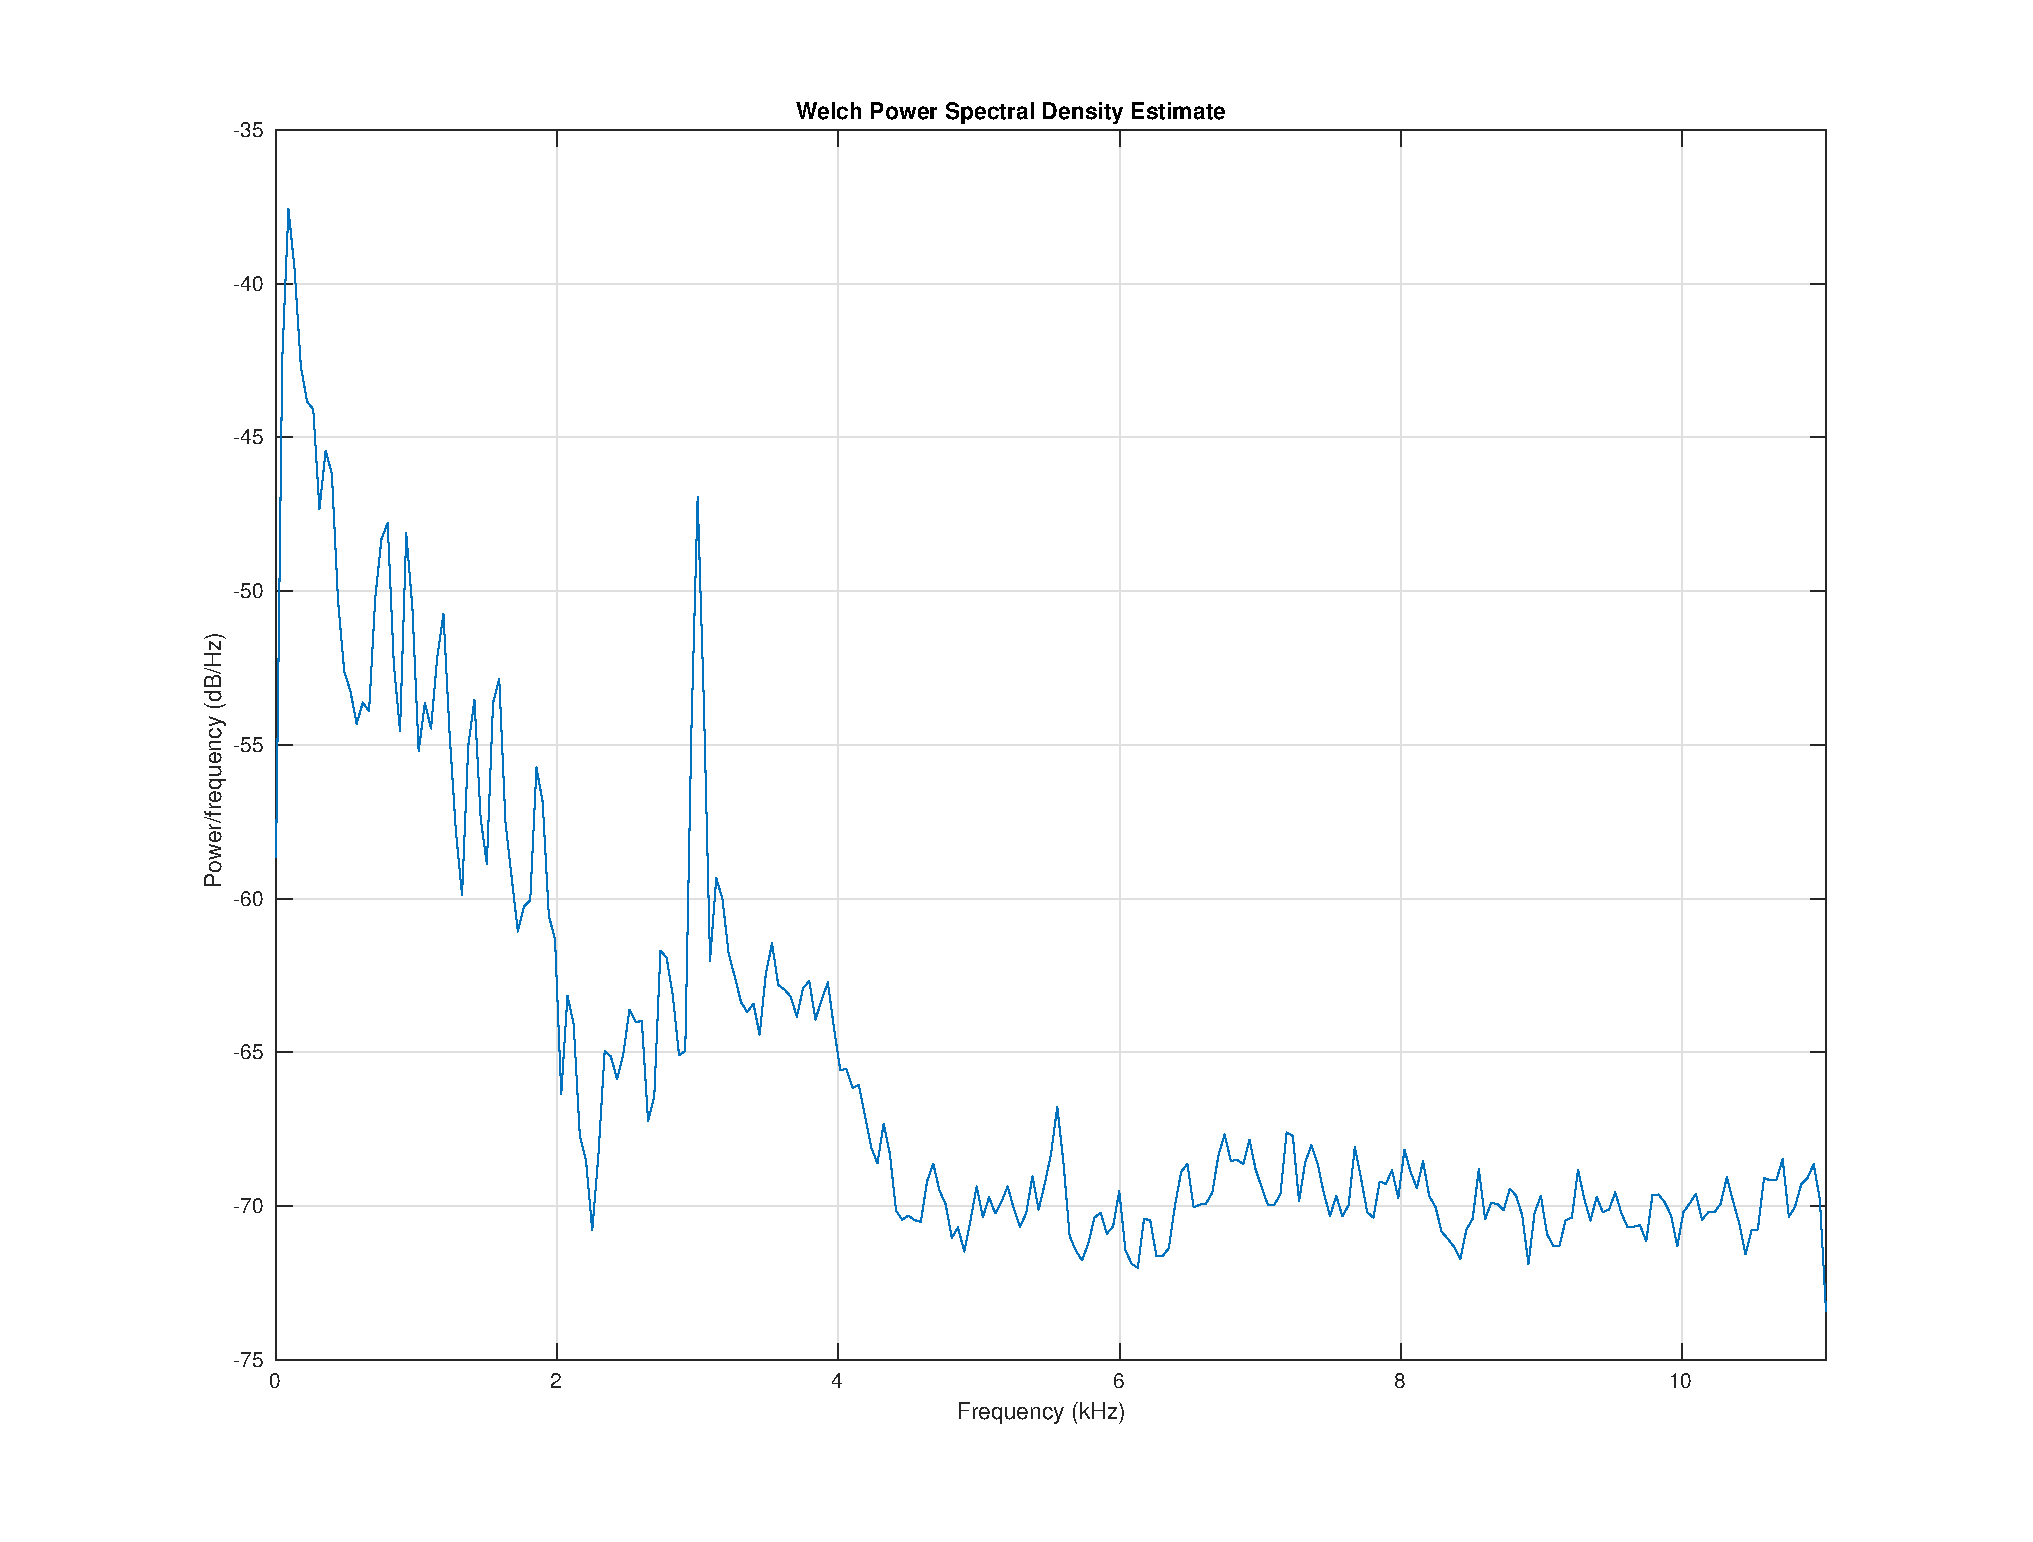
\includegraphics[width=\textwidth]{audio_freq}
        \caption{Power Spectral Density of unfiltered audio}
        \label{fig:psd1}
    \end{subfigure}
    \hfill
    \begin{subfigure}[b]{0.45\textwidth}
        \centering
        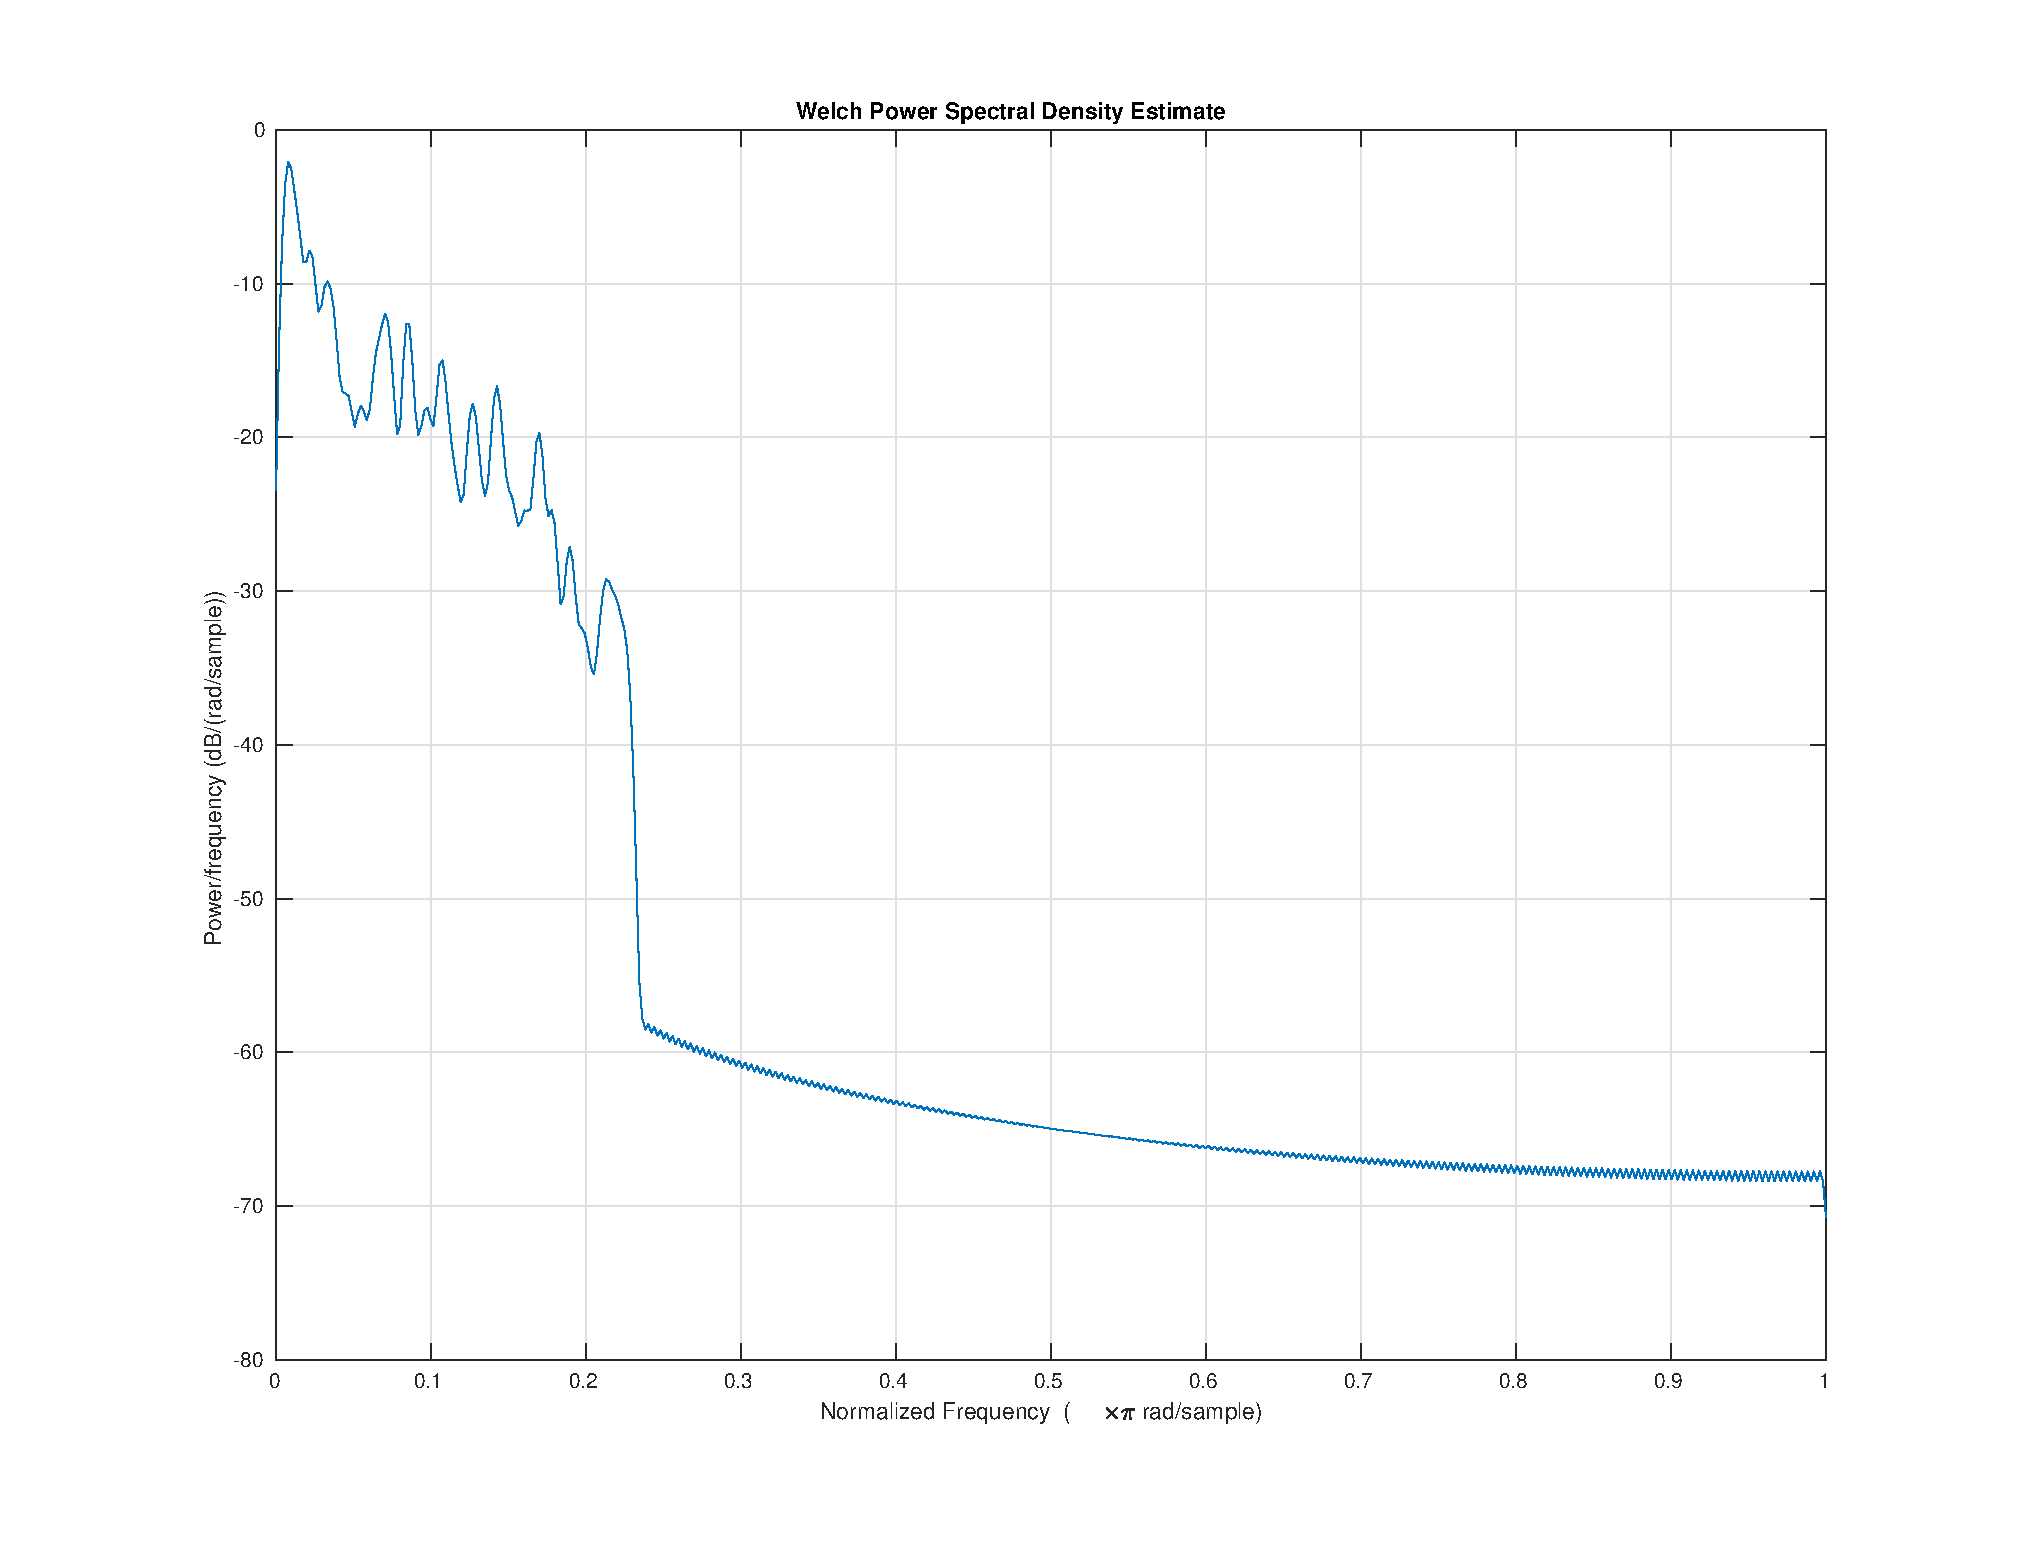
\includegraphics[width=\textwidth]{audio_lpf}
        \caption{Power Spectral Density of filtered audio}
        \label{fig:psd2}
    \end{subfigure}
    \caption{PSD plots}
\end{figure}

The 513-tap Hamming window was used to filter the audio.

With the low pass filter, mostly instruments and bass can be heard in the audio, and almost none of the singing is audible. The ringing noise is also removed.

\subsection*{High Pass Filter}

\begin{figure}[H]
    \centering
    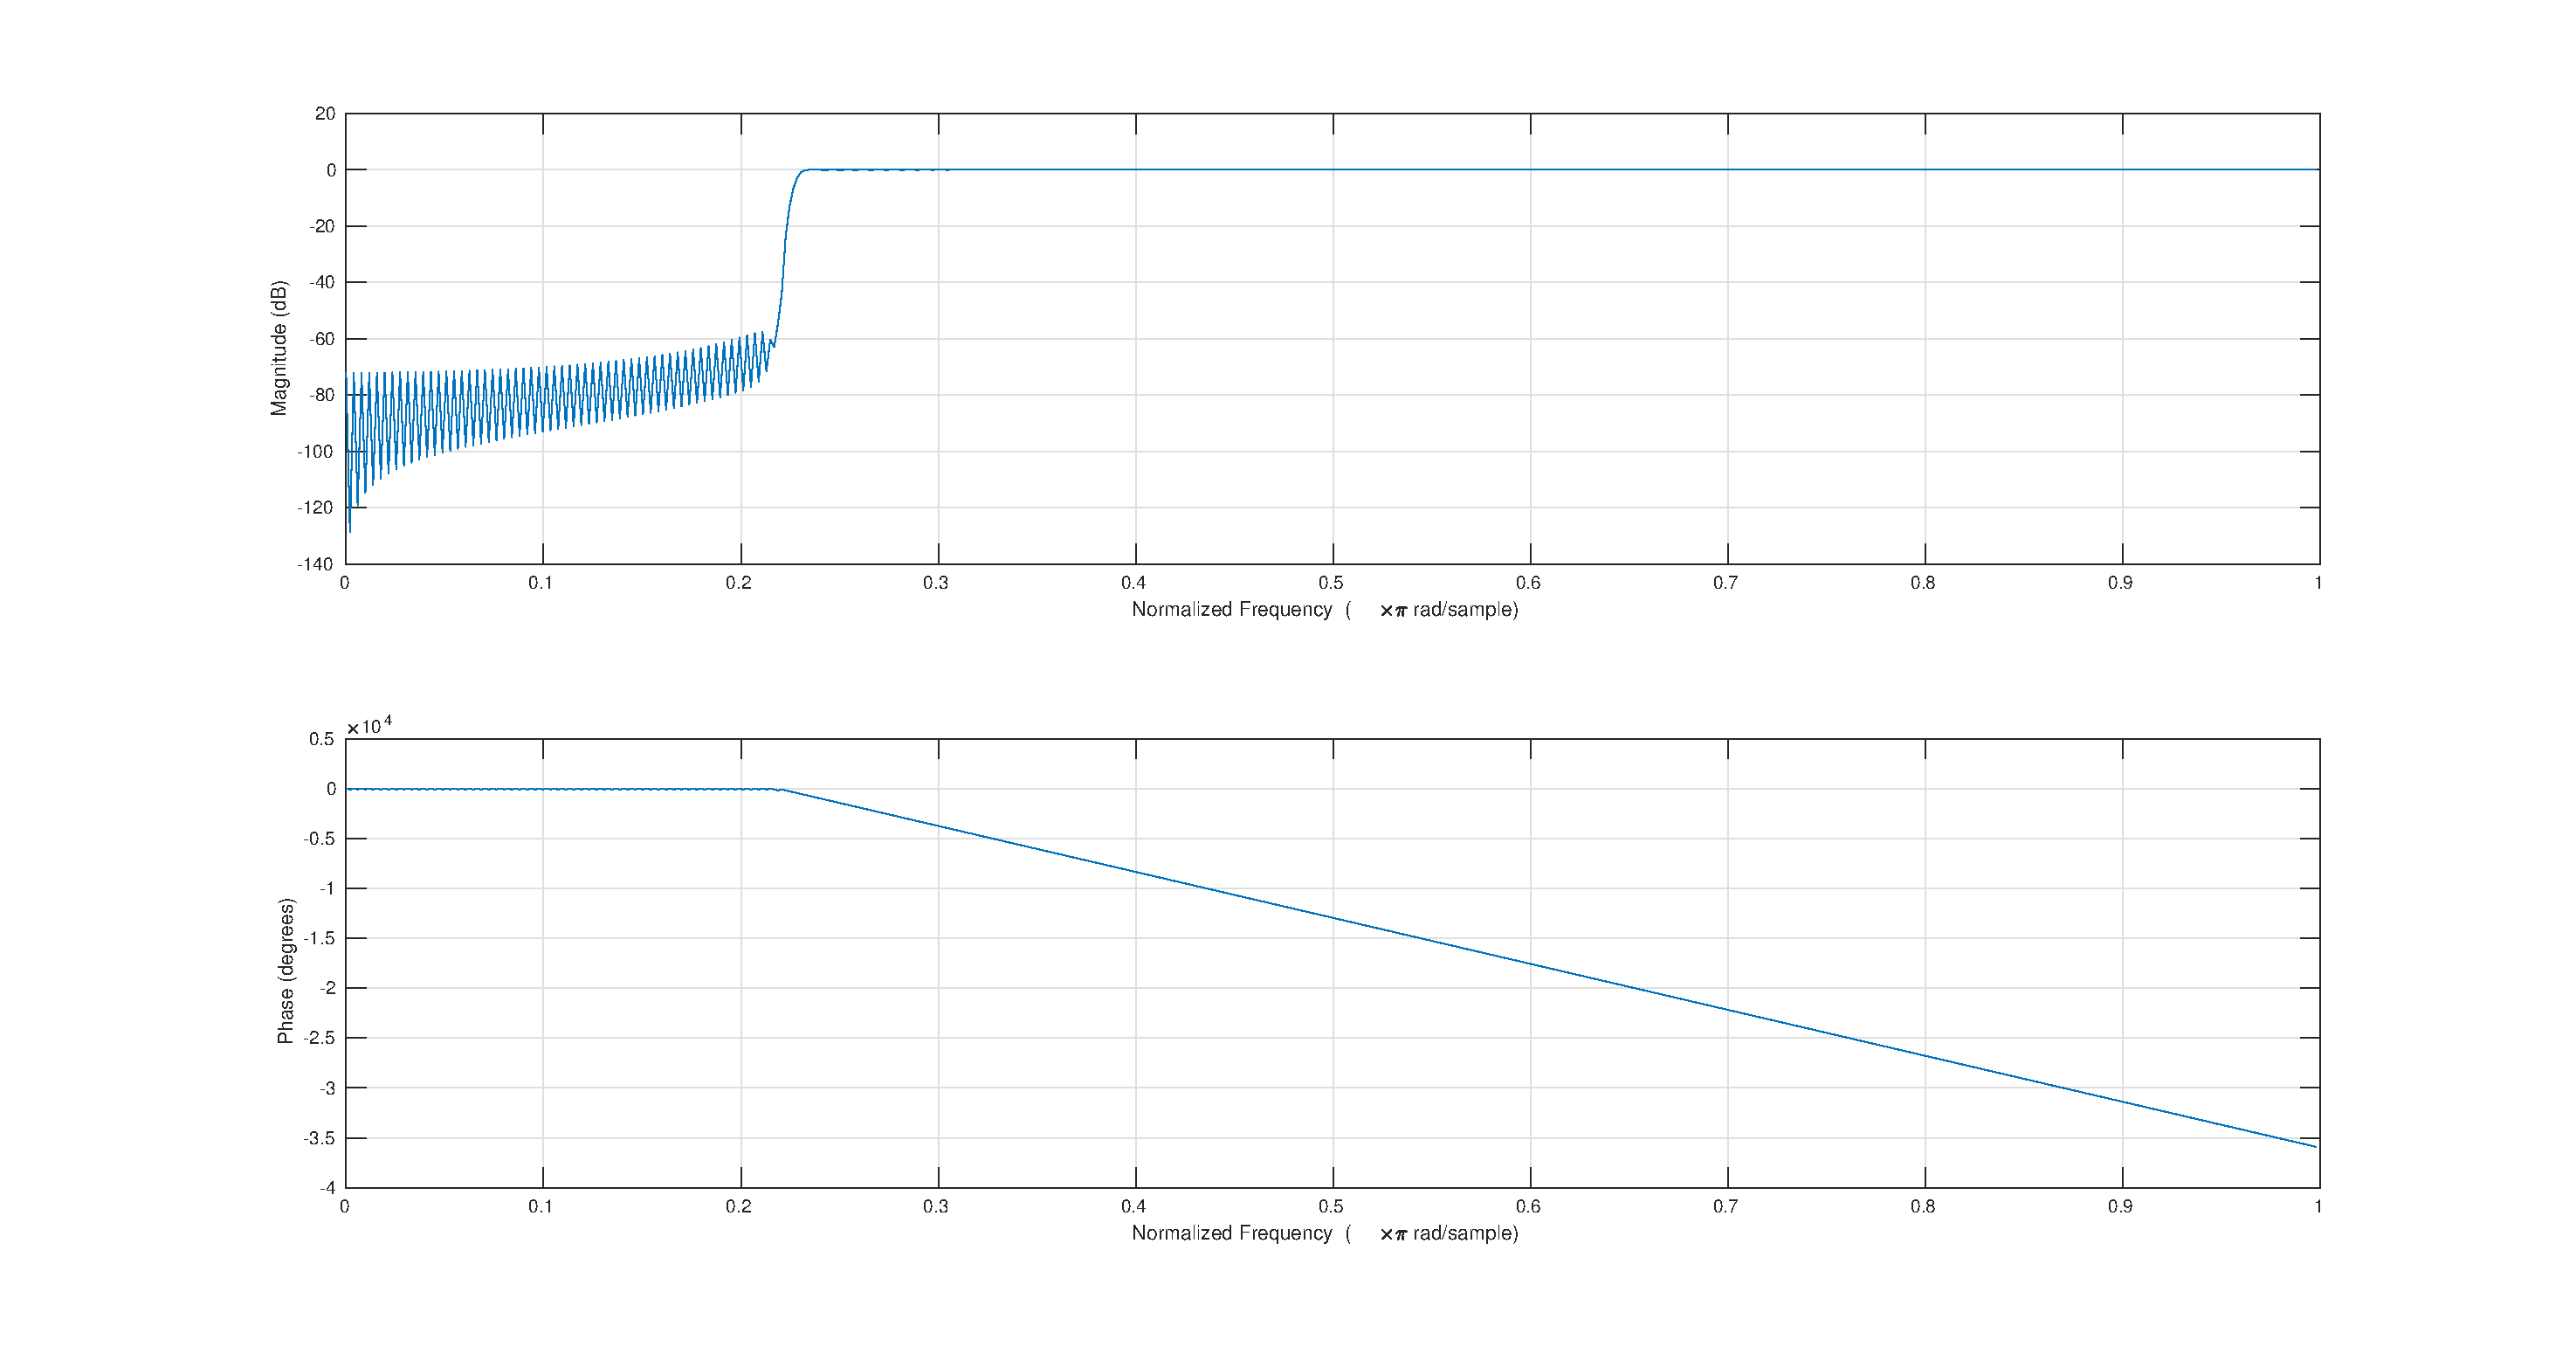
\includegraphics[width=\textwidth]{hamming_hpf}
    \caption{Frequency response of Filter}
    \label{fig:filt2}
\end{figure}

\begin{figure}[H]
    \centering
    \begin{subfigure}[b]{0.45\textwidth}
        \centering
        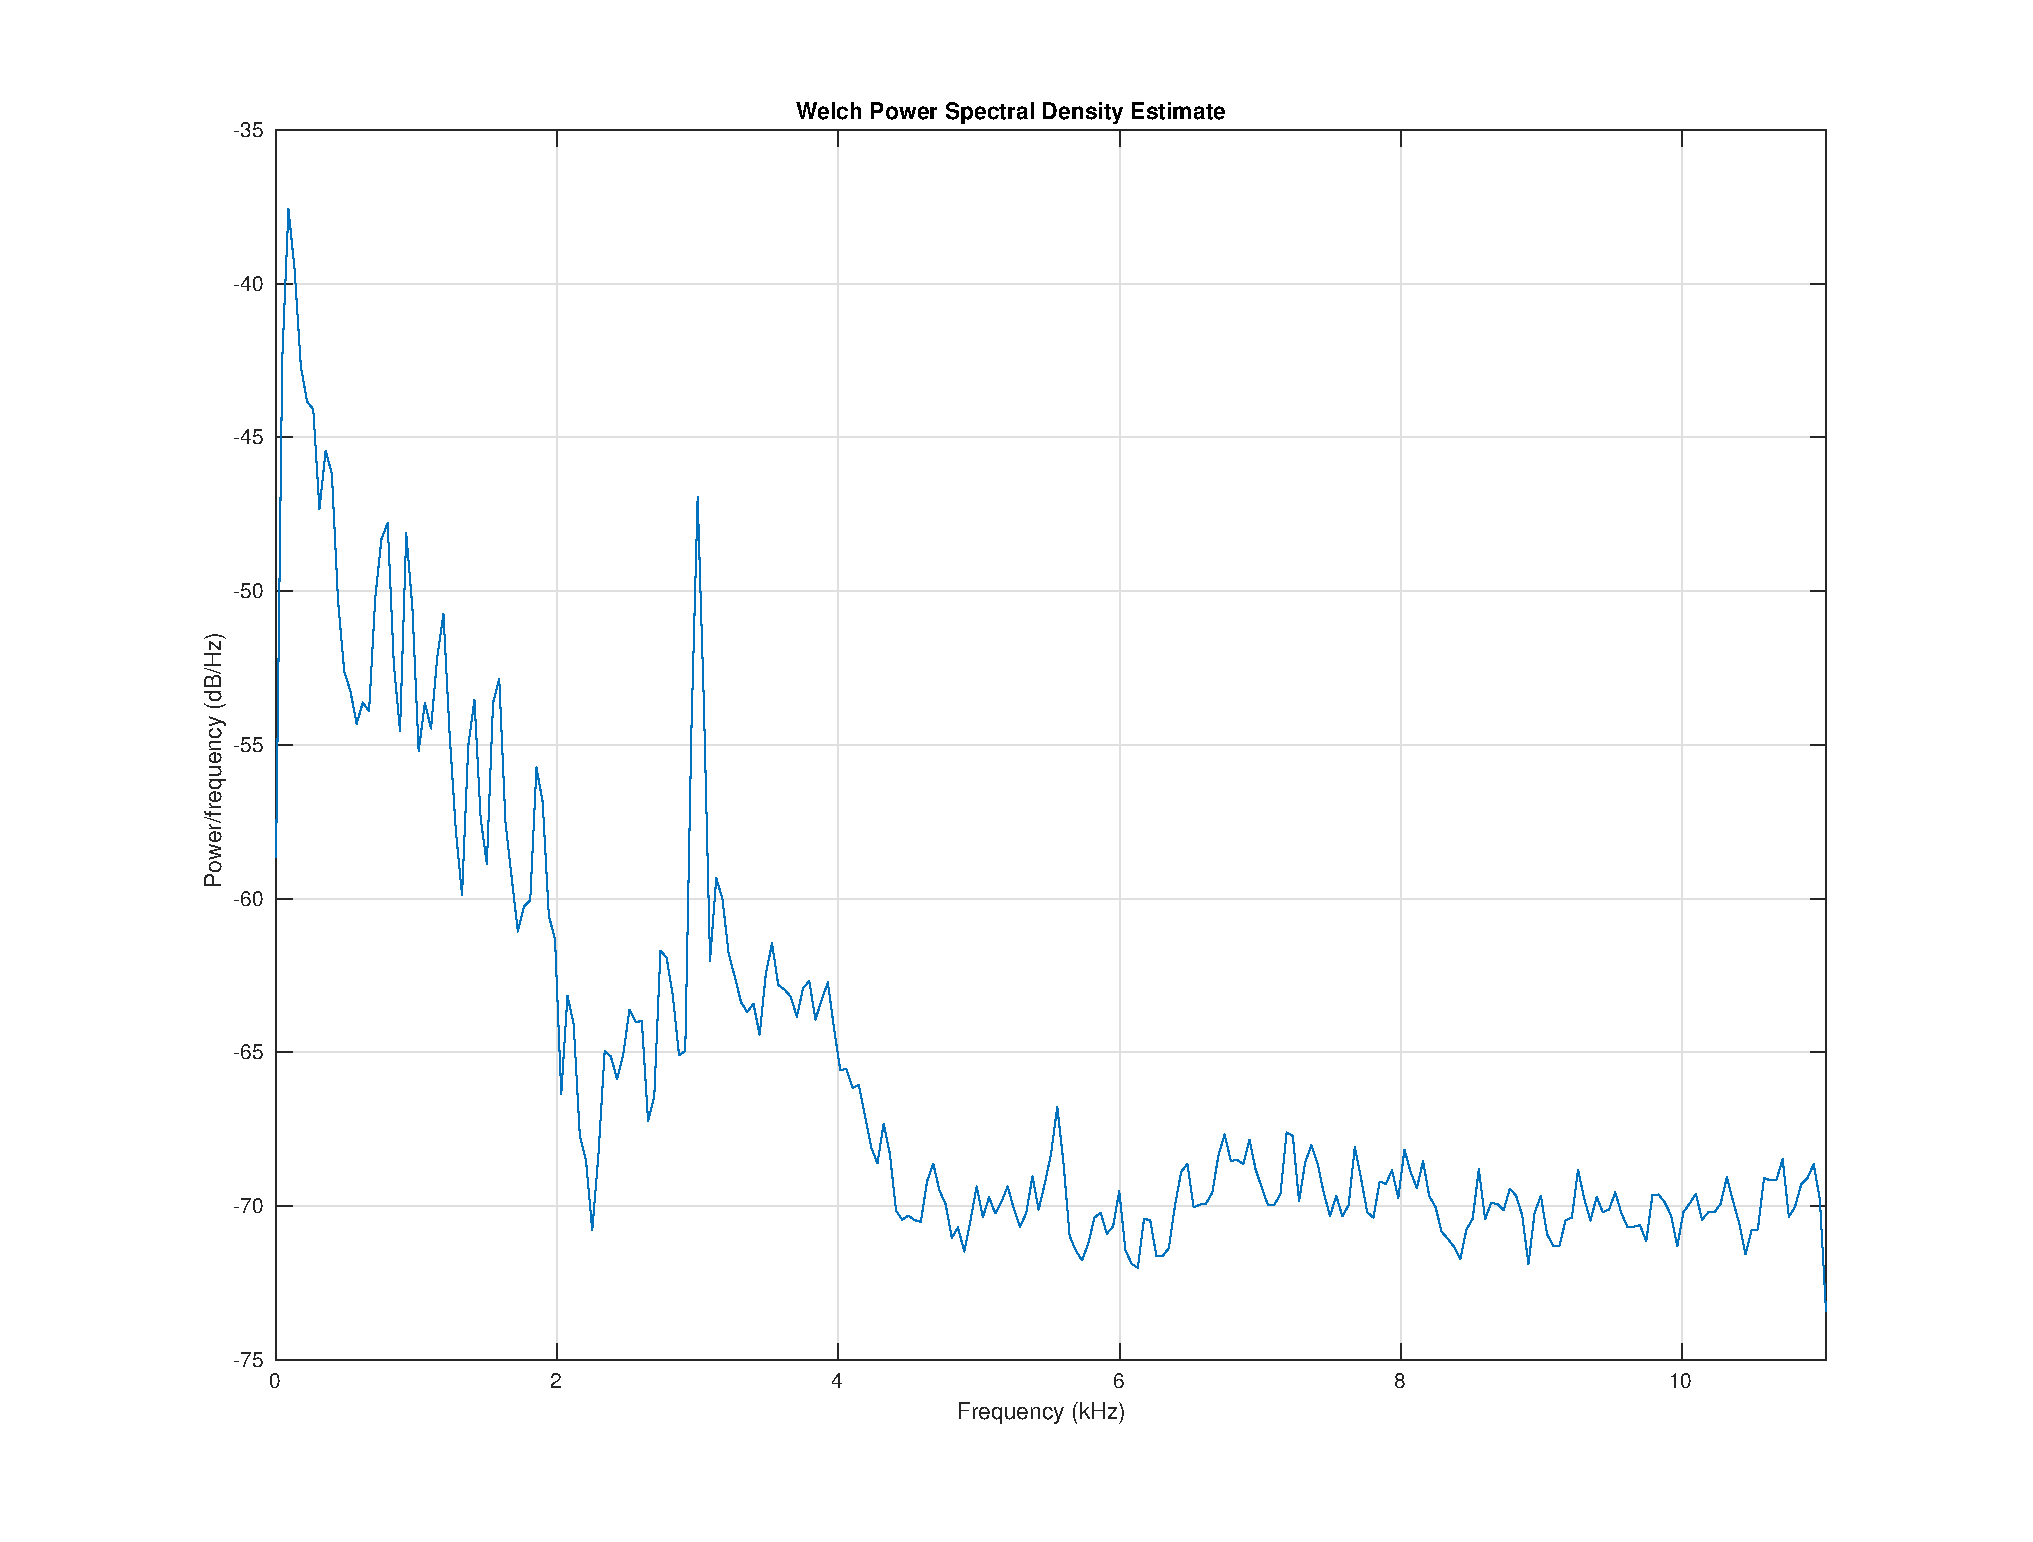
\includegraphics[width=\textwidth]{audio_freq}
        \caption{Power Spectral Density of unfiltered audio}
        \label{fig:psd3}
    \end{subfigure}
    \hfill
    \begin{subfigure}[b]{0.45\textwidth}
        \centering
        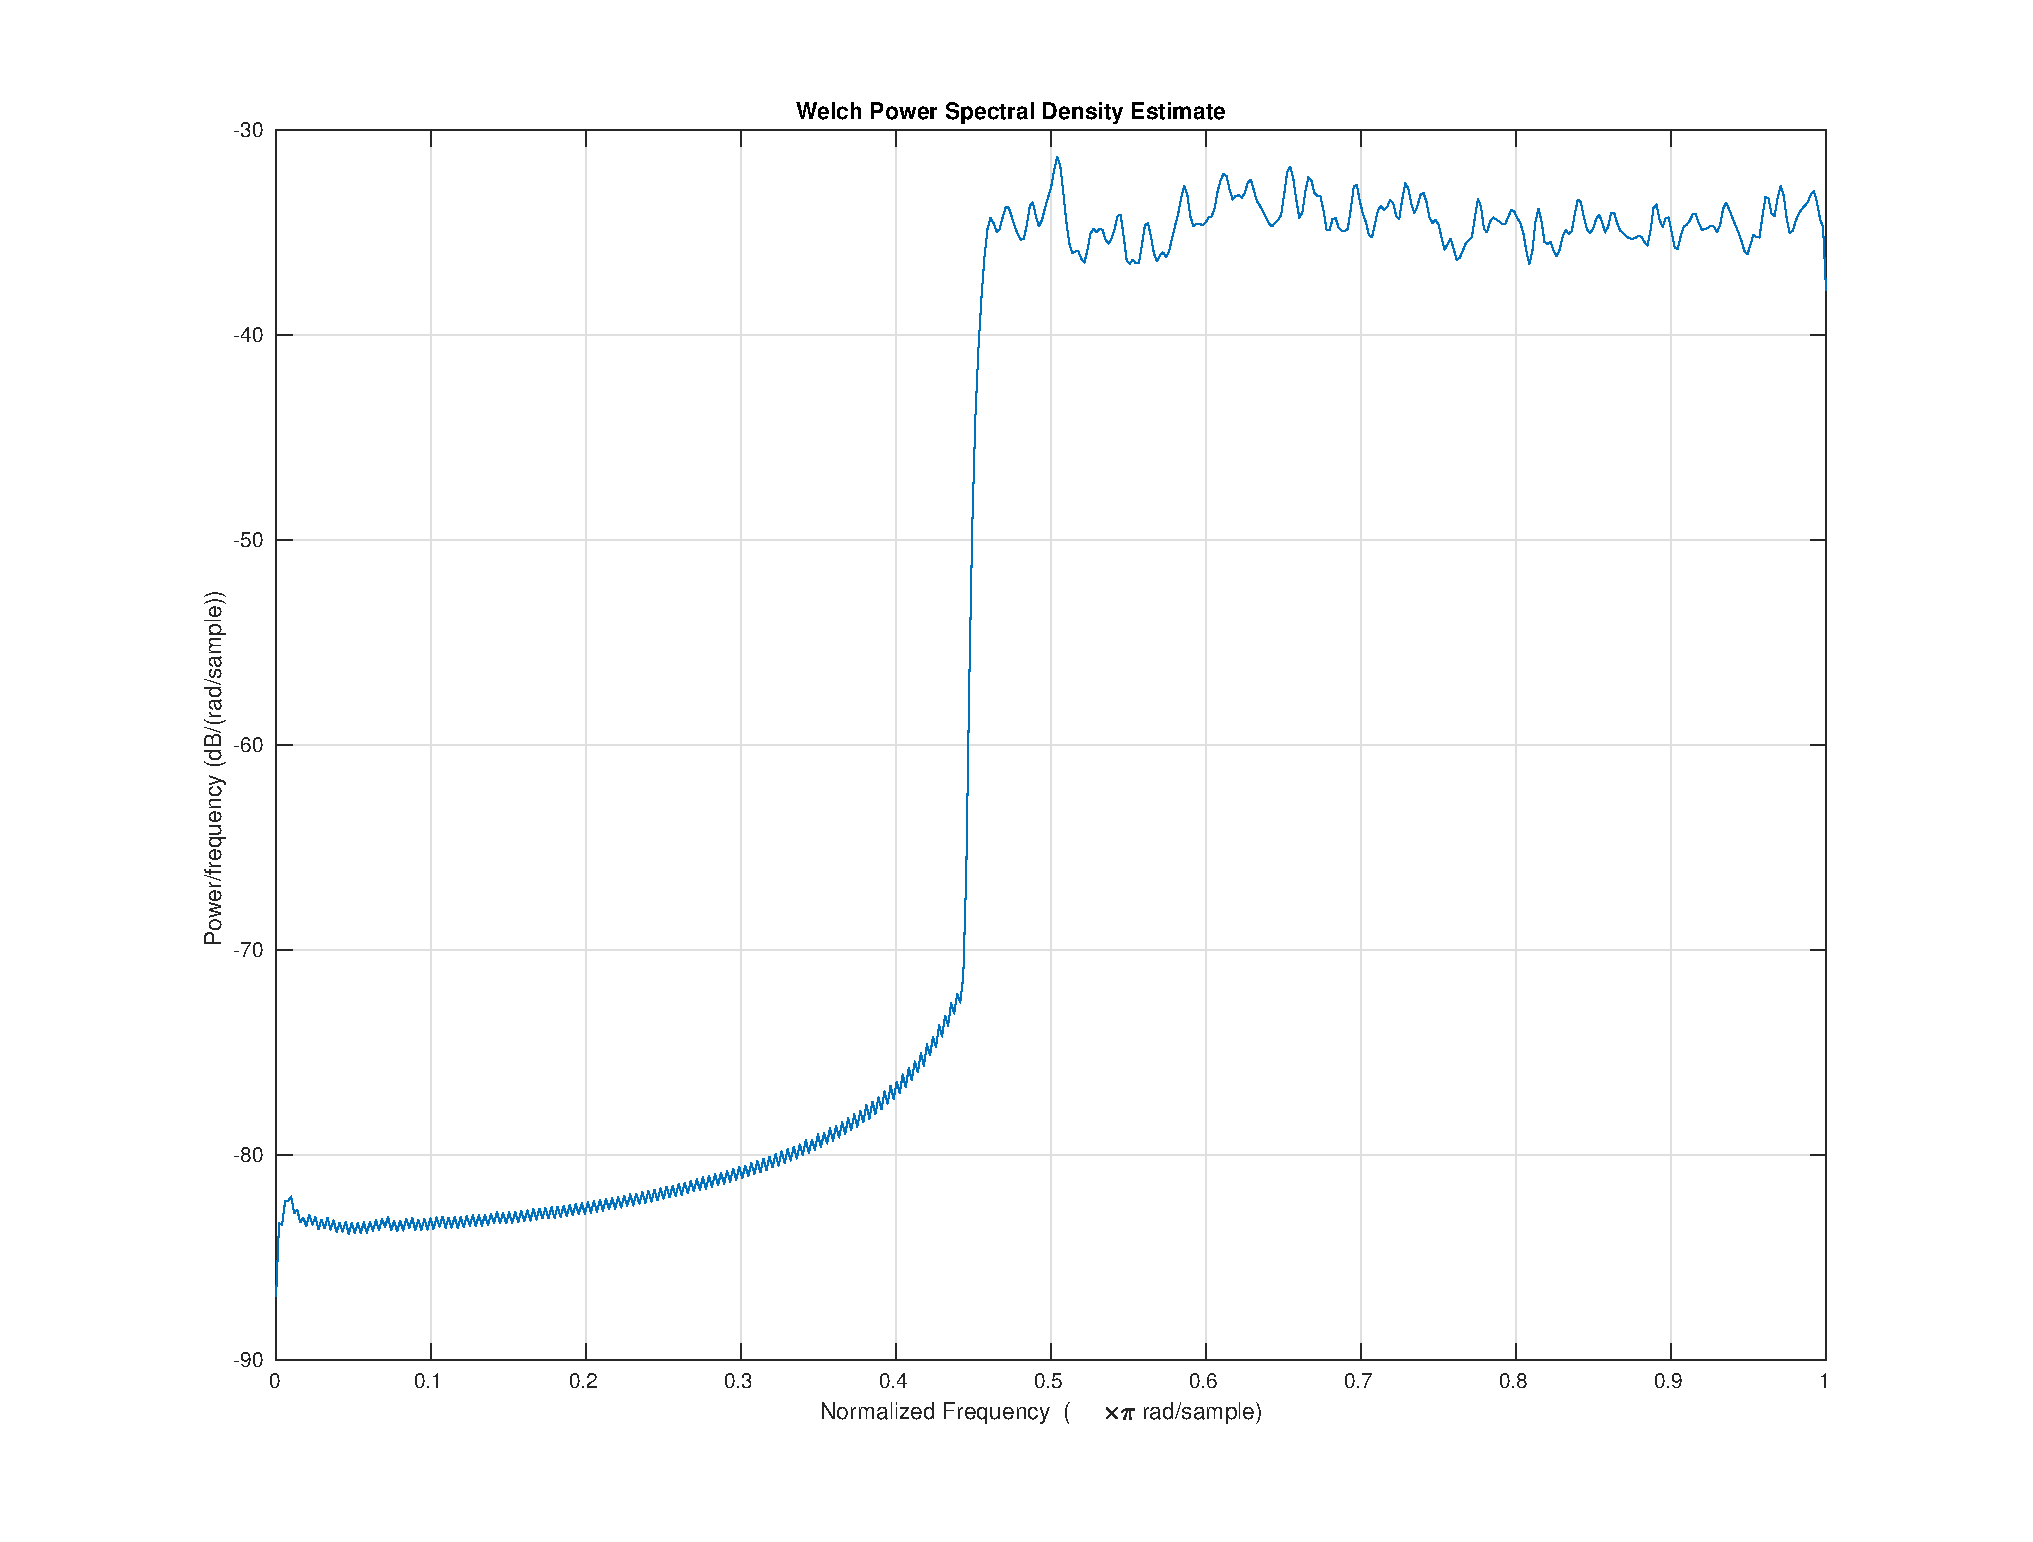
\includegraphics[width=\textwidth]{audio_hpf}
        \caption{Power Spectral Density of filtered audio}
        \label{fig:psd4}
    \end{subfigure}
    \caption{PSD plots}
\end{figure}

The 513-tap Hamming window was used to filter the audio.

With the high pass filter, some of the singing is audible and some high frequency hissing too. The ringing noise is also removed.

\subsection*{Band Pass Filter}

\begin{figure}[H]
    \centering
    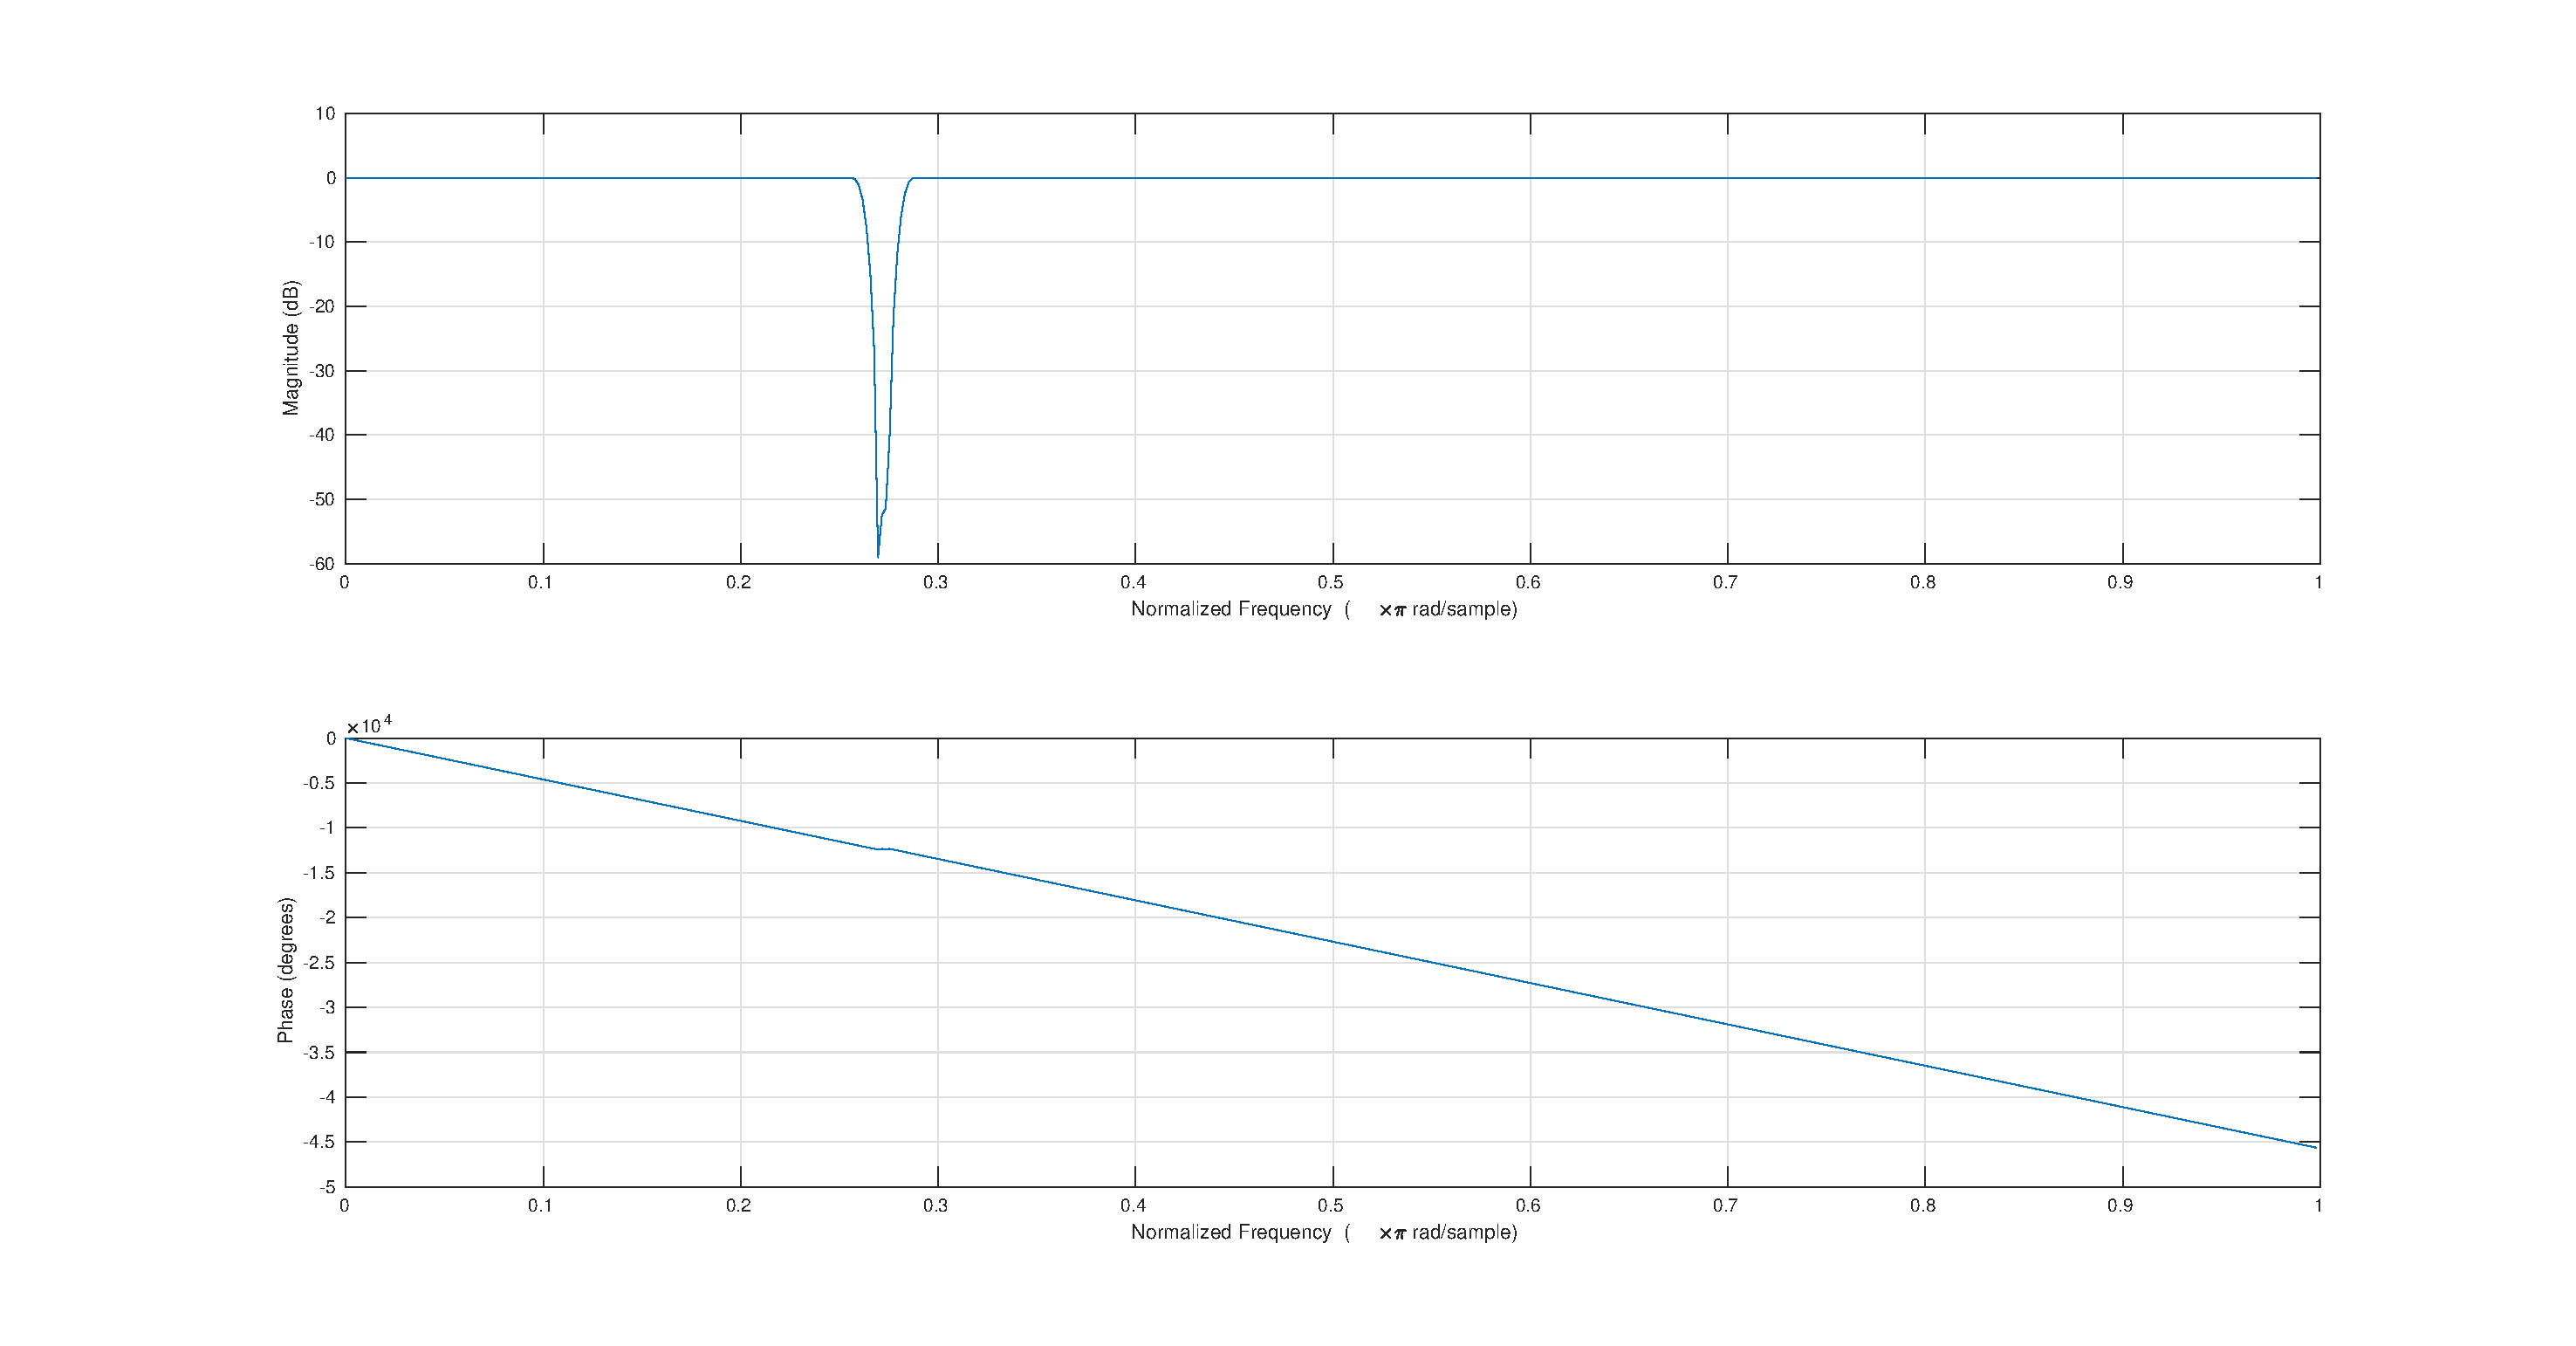
\includegraphics[width=\textwidth]{hamming_bsf}
    \caption{Frequency response of Filter}
    \label{fig:filt2}
\end{figure}

\begin{figure}[H]
    \centering
    \begin{subfigure}[b]{0.45\textwidth}
        \centering
        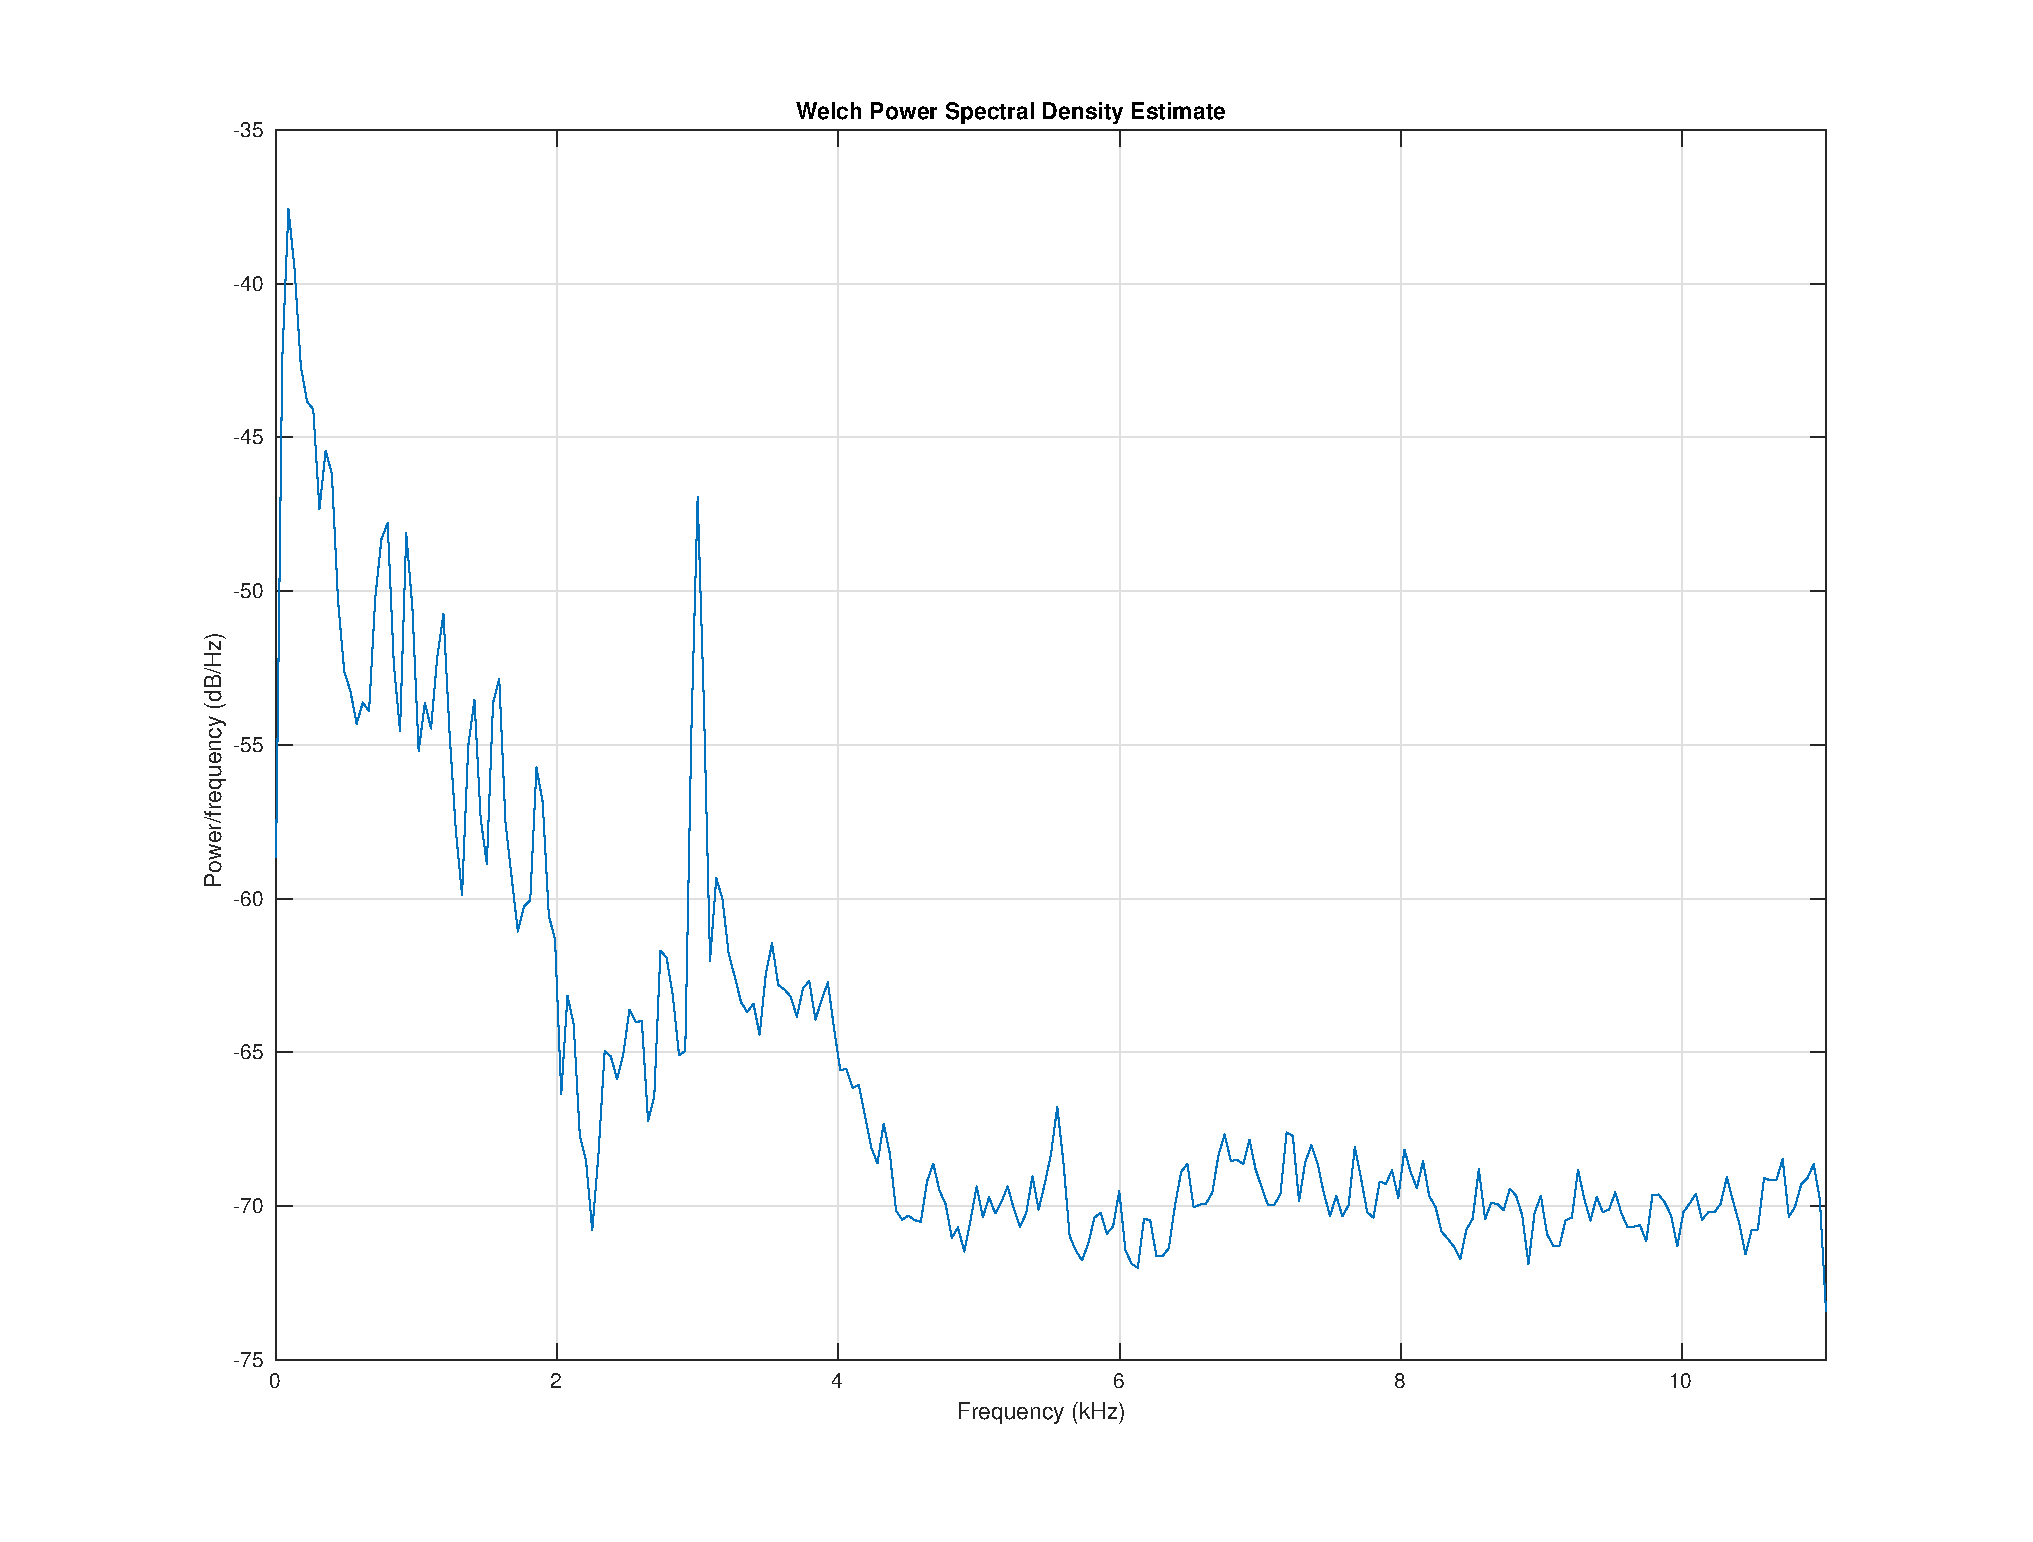
\includegraphics[width=\textwidth]{audio_freq}
        \caption{Power spectral density of unfiltered audio}
        \label{fig:psd3}
    \end{subfigure}
    \hfill
    \begin{subfigure}[b]{0.45\textwidth}
        \centering
        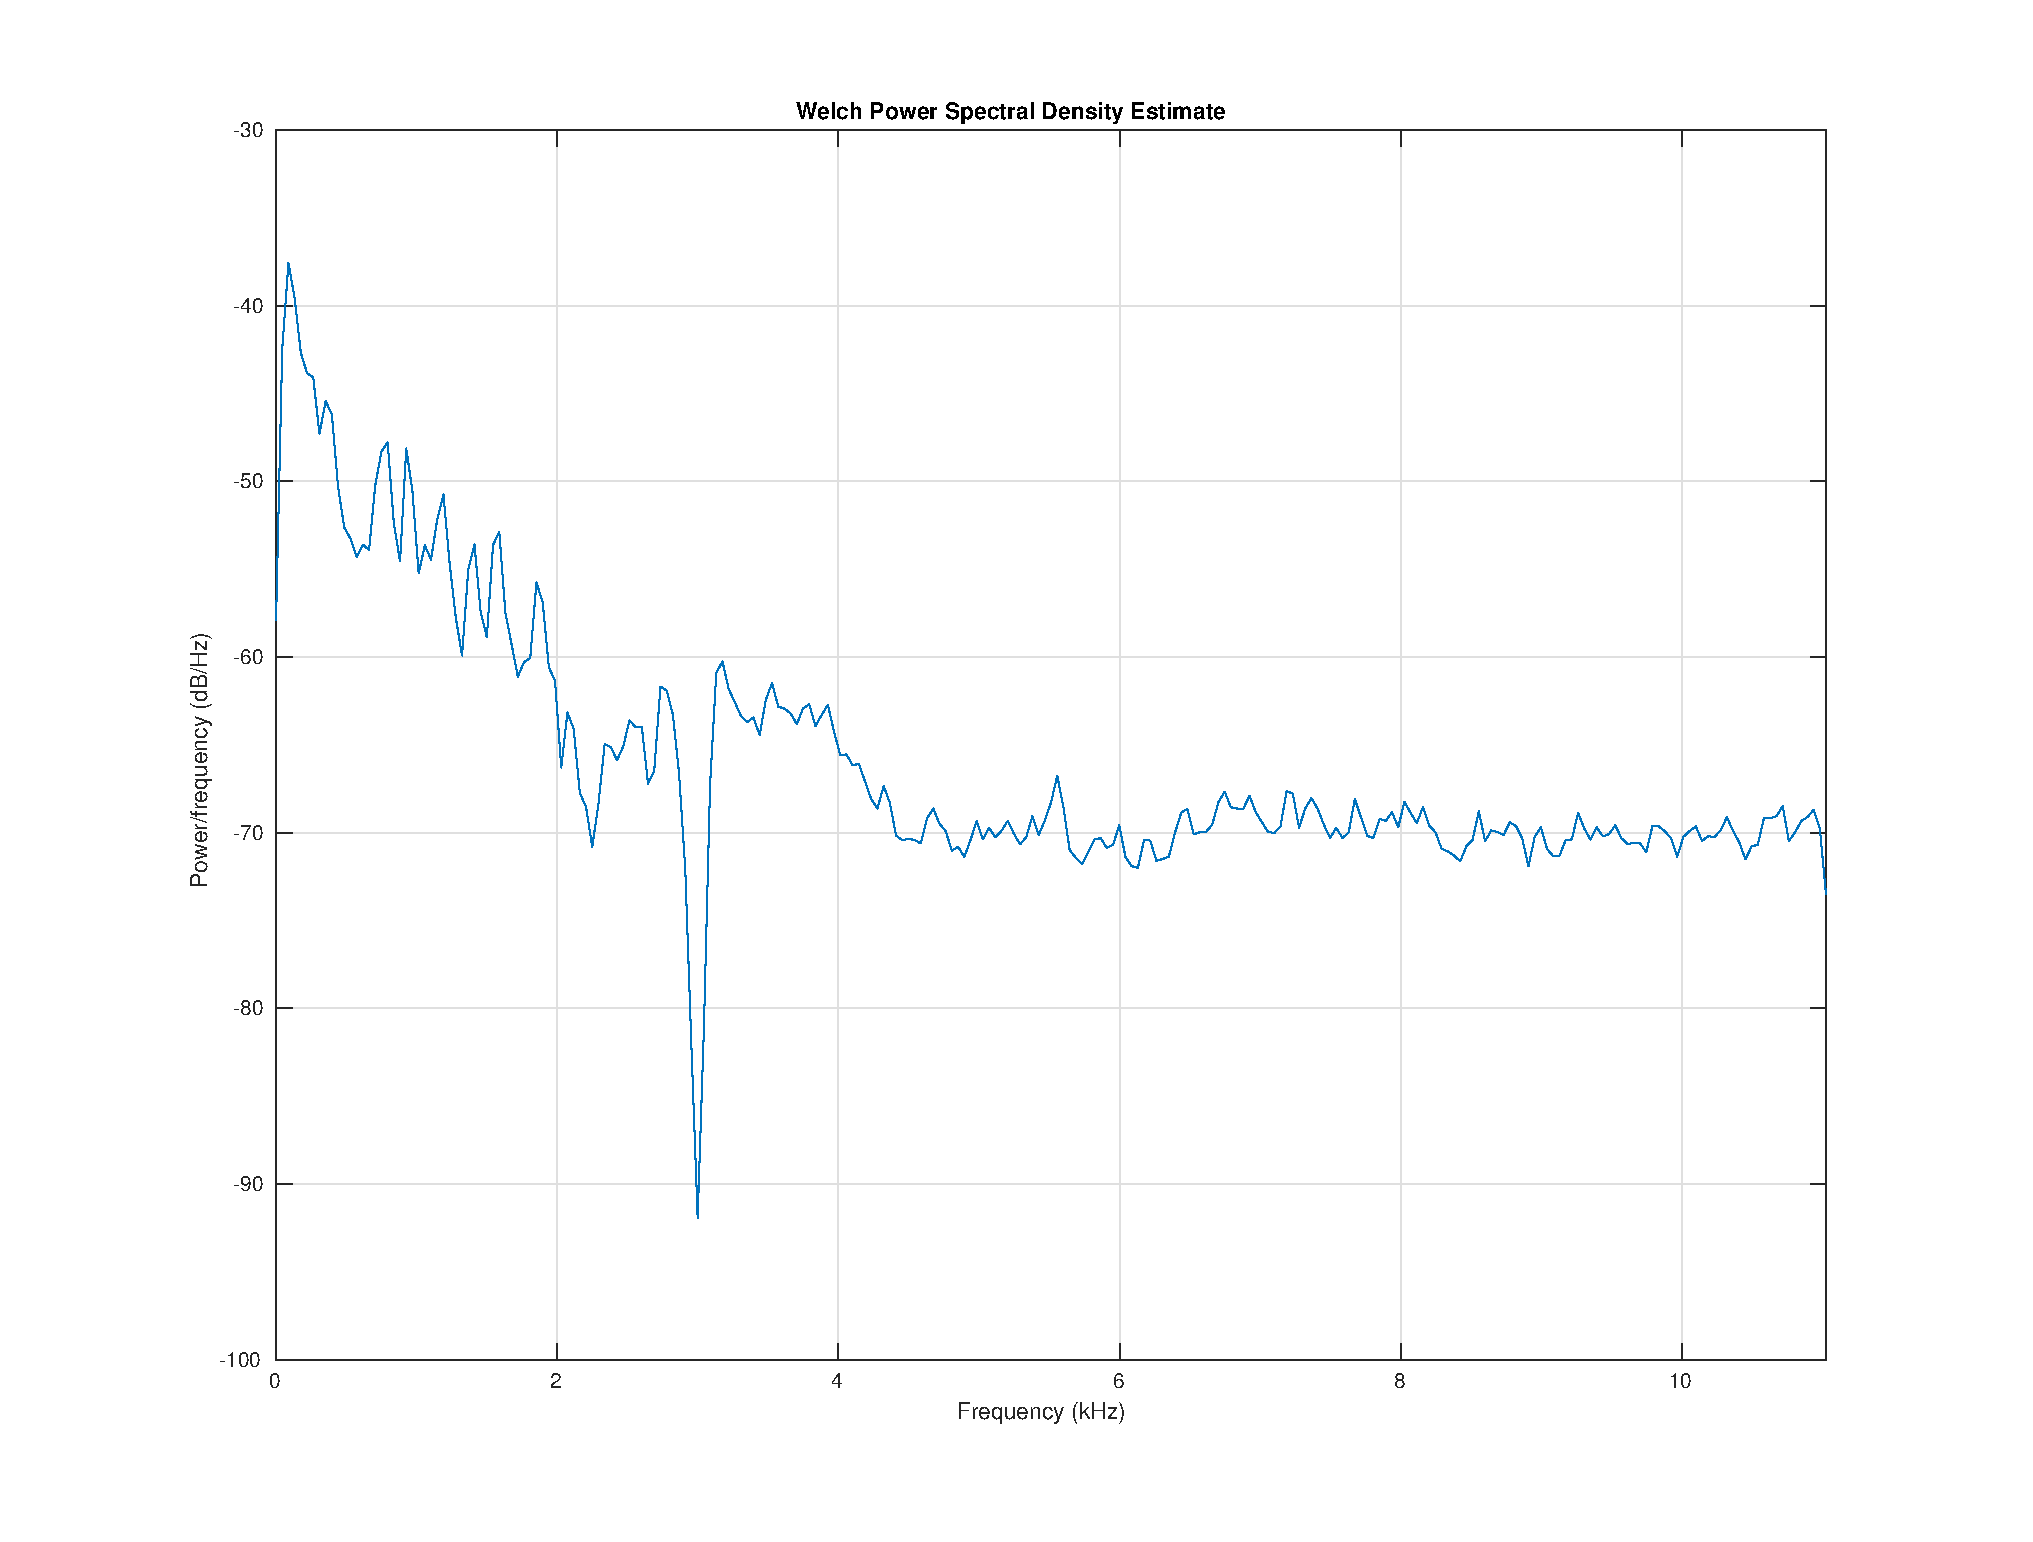
\includegraphics[width=\textwidth]{audio_bsf}
        \caption{Power spectral density of filtered audio}
        \label{fig:psd4}
    \end{subfigure}
    \caption{PSD plots}
\end{figure}

The 513-tap Hamming window was used to remove the ringing noise from the audio.

With the band stop filter, all of the song is audible, and only the ringing noise is removed.
\section{Image Filtering}

\begin{figure}[H]
    \centering
    \begin{subfigure}[b]{0.45\textwidth}
        \centering
        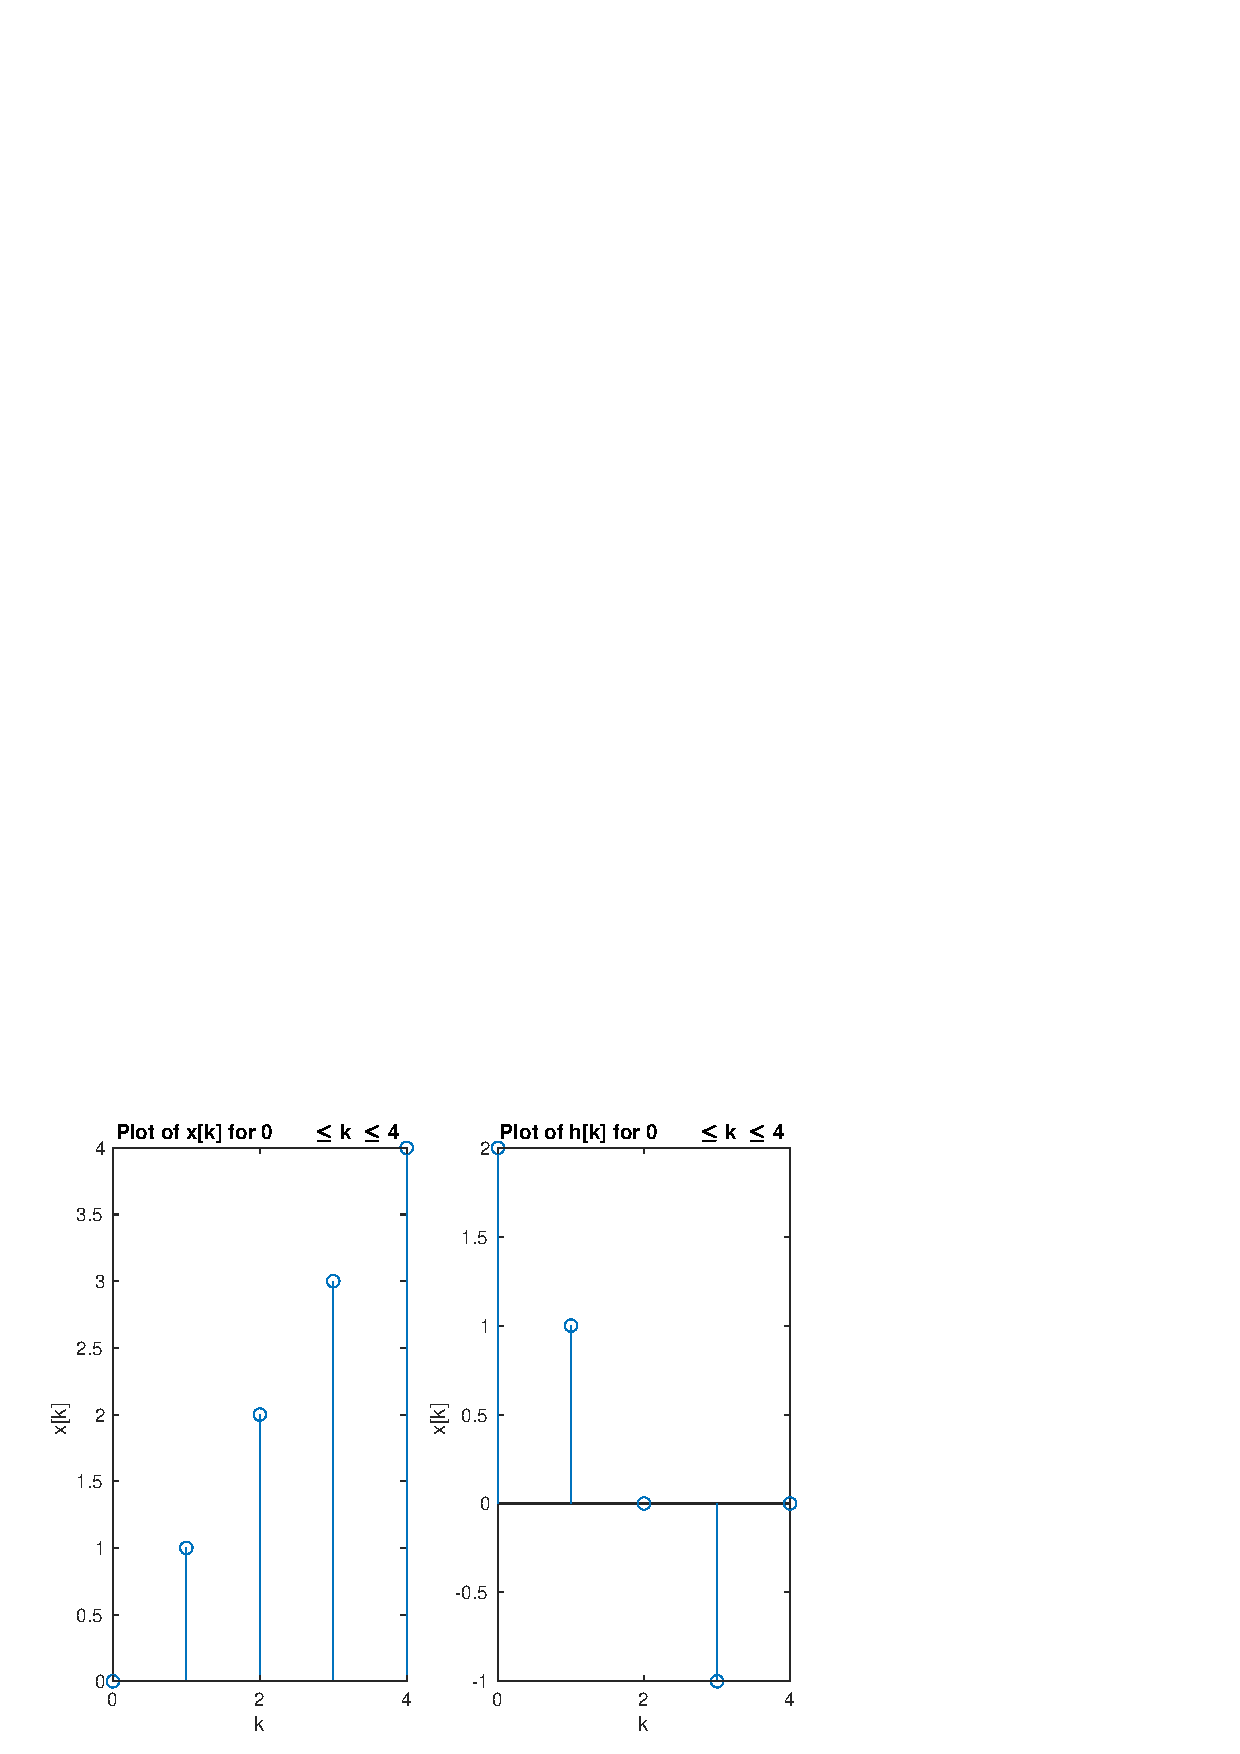
\includegraphics[width=\textwidth]{plot1.png}
        \caption{Power spectrum of the image}
    \end{subfigure}
    \hfill
    \begin{subfigure}[b]{0.45\textwidth}
        \centering
        \includegraphics[width=\textwidth]{plot.png}
        \caption{Frequency response of the filter}
    \end{subfigure}
    \caption{PSD plots}
\end{figure}

\verb|plot1.tiff| represents the power spectral density of the image, while \verb|plot.tiff| shows the frequency response of the filter applied to the image. When the filter is applied to the image, it is through the operation of convolution, and what the filter's response is showing is that the middle pixel of the current block being processed is weighted heavily, and surrounding pixels are taken into account slightly, but not as much as the one in the middle.


\begin{figure}[H]
    \centering
    \begin{subfigure}[b]{0.45\textwidth}
        \centering
        \includegraphics[width=\textwidth]{ayantika.png}
        \caption{Original image}
    \end{subfigure}
    \hfill
    \begin{subfigure}[b]{0.45\textwidth}
        \centering
        \includegraphics[width=\textwidth]{ayantika_filt.png}
        \caption{Filtered image}
    \end{subfigure}
    \caption{PSD plots}
\end{figure}

As shown above, the filtered image is darker. This is due to the filter's sampling amplitude. The middle pixel is sampled at about 0.5 times it's original brightness. Due to the way the filter takes a block of pixels into account, each pixel is not what it was before, but a weighted average of the surrounding pixels. The end result is that the produced image is also about half the brightness and is much blurrier.

\pagebreak
\appendix
\section{Complete Code}
\inputminted{Matlab}{Lab5.m}

\pagebreak
\section{Question 4 Code}
\inputminted{Matlab}{Lab5Q4.m}

\end{document}
